%%%%% Beginning of preamble %%%%%
\documentclass[12pt]{article} 

%What kind of document (article) and what size
%Packages to load which give you useful commands
\usepackage{amssymb, amsmath, amsthm} 
\usepackage{epsfig,graphicx} 
\usepackage{caption}
\usepackage{subcaption}


%Sets the margins
\textwidth = 6.5 in 
\textheight = 9 in 
\oddsidemargin = 0.0 in 
\evensidemargin = 0.0 in 
\topmargin = 0.0 in 
\headheight = 0.0 in 
\headsep = 0.0 in \parskip = 0.2in \parindent = 0.0in

\begin{document} 

\section{Community Structure}

Many real networks have 
a natural community structure, where disjoint subgroups of nodes exchange many internal 
connections among then than with the rest of nodes. Formally, we want to compute the optimal 
division of the network that minimizes the number of links between subgroups (also called 
communities). The raw number of links at the boundary does not give a good partition of the 
network. For example, the community structure can be a consequence of random variations in
the density of links (2). A more reliable approach uses a null model to assess the quality of a 
given network partition. Newman and Girvan \cite{newman2004finding} defines the modularity as follows:

\begin{equation}
Q = \frac{1}{2m} \sum_{ij} \left( A_{ij} -
\frac{k_i k_j}{2m} \right) \delta(g_i,g_j)
\label{eq.q}
\end{equation}

where $2m = \sum_{ij} A_{ij}$ is the number of links and $g_i$
gives the label of the community the node $i$
belongs to. Notice that maximizing the above function yields a partition that minimizes the 
expected number of links falling between different communities, i.e., when 
$\delta(g_i, g_j) = 0$. 
Modularity $Q$ takes values between 0 and 1: low modularity indicates the number of links 
between distinct communities is not significantly different from the random distribution and high 
modularity indicates there is a strong community structure.

\section{Community detection in a single layer}

We analyzed the real twitter data using two the binary
and the weighted version of the adjacency matrix using
a Matlab version of the Louvain algorithm \cite{blondel2008fast}.
The results are (confirming Elisa's values):

\begin{center}
	\begin{tabular}{ | r | c | c |}
		\hline
		& Binary & Weighted\\ \hline
		$c$ & 27 & 37 \\ \hline
		$Q$ & 0.2610 & 0.4082 \\ \hline
	\end{tabular}
\end{center}

As we can see, the modularity value increase considerably from
binary to weighted representation. However, because the
representation of the network is different (binary vs weighted),
the modularity value is not enough to say that the community
structure is different. The reason of the difference in values
may be only because we chose different representations. However,
we will show in the following subsection that the community partition
is also different. 

\subsection{Distinguishing binary vs weighted community partition}

By just looking at the number of modules in each representation,
we can be tempted to say that the community structure is different.
However, as the next table shows, the percentage of total nodes
inside the biggest five nodes is very high. In other words, the
first five biggest modules dominates the community structure.


\begin{center}
	\begin{tabular}{ | r | c | c | c | c | c | c |}
		\hline
		& 1 & 2 & 3 & 4 & 5 & Total \%\\ \hline
		Binary & 1092 & 941 & 410 & 292 & 12 & 97.76 \\ \hline
		Weighted & 1098 & 938 & 220 & 293 & 140 & 95.69 \\ \hline
		Shared & 876 & 777 & 66 & 244 & 0 & 69.86\\ \hline
		
	\end{tabular}
\end{center}

First, notice that the total size (last column) of the five biggest modules very high ($>95$ \%) as already described. Second, notice
that for the binary row we sorted the modules in decreasing order.
However, for the weighted row this is not the case (see module 3 and 4).
We relabel the weighted partition in order to maximize similarity
structure with the binary partition.

\subsubsection{Jacquard's index}

The lector may already infer that the value at the right-bottom
is an estimation (based in the fact that $>95$\% of nodes are inside the five biggest modules) of the Jacquard index, which in this case
can be translated as:

\begin{equation}
J = \frac{\text{Number of nodes inside the same modules}}{\text{Total number of nodes}}
\end{equation}

\section{Community detection across time snapshots}

In addition to study the community structure a static single network, we studied how the community structure changes across time snapshots. The main reason of this analysis is that, in real twitter data,  the mutual information between users may variate across time, and therefore the community structure of the mutual information network may change across time. As
a specific example, this type of analysis could potentially be a method to detect the birth of trading topics in the twitter social network.



\subsection{Algorithms}

In order to perform the analysis we used two modularity algorithms
specifically designed either for time snapshots or multiplex networks (a time varying network
can be described as a multiplex network in which each time snapshot is a multiplex layer).
These two algorithms are described on the articles published by Kawadia and Sreenivasan
\cite{kawadia2012sequential}, and Mucha et Al \cite{Mucha14052010}. Both algorithms are available
online as open source in Python and Matlab, respectively. 

\subsubsection{Kawadia and Screenivasan algorithm}

The idea of this algorithm is to find a new community partition $P_t$ for a graph snapshot $G_t$, such that the Estrangement (a distance
metric that the authors defined) between the new partition and the
previous one is smaller than $\delta$. In other words, the algorithm optimizes
the following constrained optimization problem:

\begin{equation}
\begin{array}{l}
\operatorname*{maximize}_{P} \hfill Q(P)\\
\operatorname*{subject\, to} \hfill E(P) \le \delta,
\end{array} 
\label{eq.opt}
\end{equation}
where $E(P)$ represents the estrangement between the current
and the last community partition. The authors make use a Lagrange
multiplier to solve this problem (for more details see \cite{kawadia2012sequential}). Unfortunately, even that the algorithm
worked for the synthetic data, it did not for the real twitter
data. The reason is that the Python library that
they use to solve the constraint satisfaction problem becomes really
slow for networks of big size as is the case of the real twitter data
that we present here.

\subsubsection{Mucha et Al algorithm}

This algorithm is based in optimizing a modularity definition that
includes extra terms for the existence of different network layers,
which in this case consist of different time snapshots. The new
modularity definition that the authors propose to optimize
in order to find the change of modularity across layers is:

\begin{equation}
Q_{multilayer} = \frac{1}{2\mu} 
\sum_{ijsr} \left\{ \underbrace{ \left( 
A_{ijs}
 - \gamma_s \frac{k_{is} k_{js}}{2m_s}\right) \delta_{sr} 
 }_{\text{within layer contribution}}
 + \underbrace{\delta_{ij} C_{jsr}}_{\text{between layer contr.}}
 \right\} \delta(g_{is},g_{jr})
\label{eq.q.layers}
\end{equation},


where $A_{ijs}$ is the element $i,j$ of the adjacency matrix of layer
$s$, $k_{is}$ the degree of node $i$ inside layer $s$, $m_s$ the
total weight of layer $s$, $g_{is}$ the module index of node $i$ inside
layer $s$. Finally, the user parameters $\gamma_s$ balances
the within layer contribution and $C_{jsr}$ balances the
between layer contribution. $C_{jsr}$ can be seen as a virtual
link between node $j$'s of two different layers $s$ and $r$.

In order to optimize the modularity equation, the authors use
a generalization of the Louvain algorithm \cite{blondel2008fast}, which
is one of the most used when dealing with big scale networks.
The released matlab library of this algorithm outperformed
by far the previous one in terms of performance and speed. Therefore,
this algorithm is the one that we used to find how modularity
changes across time.

\subsection{Data}

We create seven different time snapshots of the twitter data, each corresponding to a different week.

\subsection{Results}

Figure \ref{fig.time.modular} represent the modularity across the
seven different weeks for a single combination of parameters. This Figure shows, that in essence, the
structure does not variate across times. This fact tell us that
for this data it may be better to just evaluate the modularity
of a single snapshot across the entire seven weeks. 

\begin{figure}
	\centering
	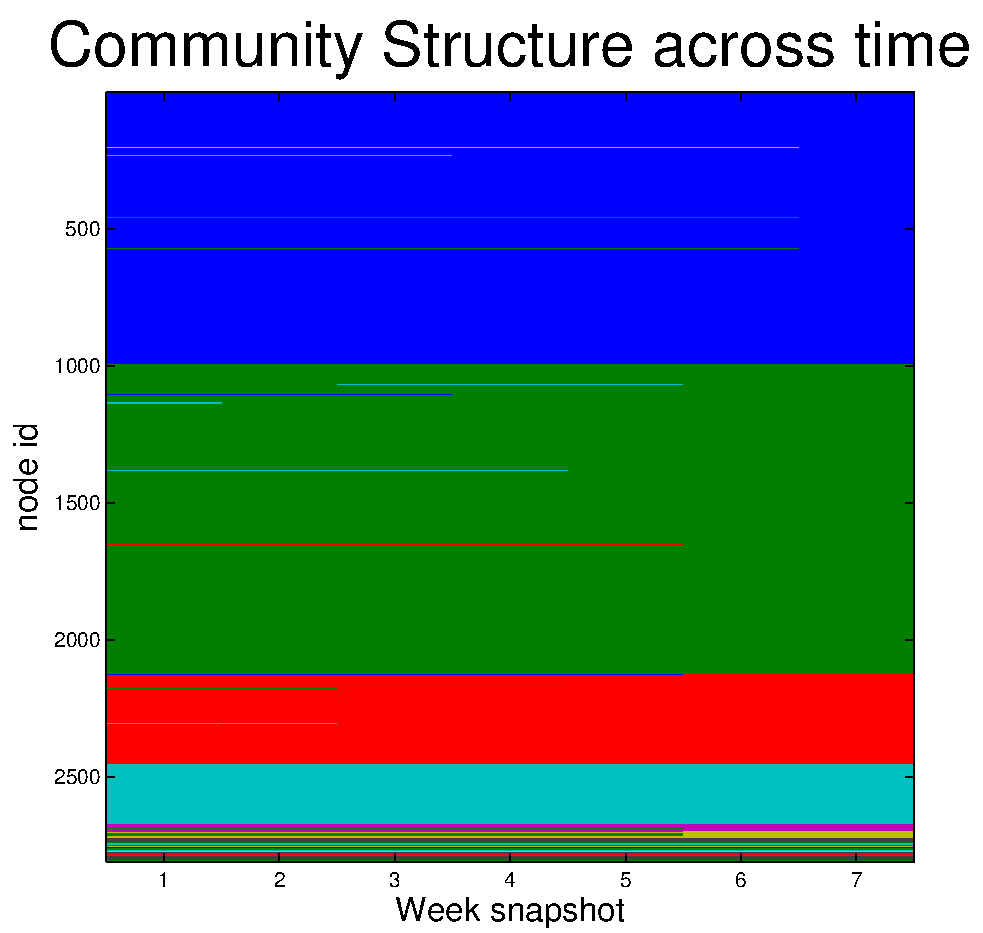
\includegraphics[width=0.87\textwidth]{Figures/modularity_time}
	\caption{Modularity across time with parameters
		$\gamma_s$ = 1 for all $s$ and $C_{jrs} = \omega=0.25$ for
		all $j,s,r$.
		 Different colors represent
		the module id to which each node (rows in this figure)
		belong to. We can observe, that the structure is dominated
		by the existence of four big modules plus a lot of small
		size modules (bottom of the Figure). Further, the modularity
		structure remains almost constant across time in the sense
		that only a very small number of nodes (represented as colored
		lines inside the big modules) switch to other modules as
		time develops.}
	\label{fig.time.modular}
\end{figure}
	


\bibliographystyle{plain}
\bibliography{../references}

\end{document}